\documentclass[11pt]{article}
\usepackage[margin=1in]{geometry}
\usepackage{amsmath,amssymb}
\usepackage{booktabs}
\usepackage{xcolor}
\usepackage{hyperref}
\usepackage{tikz}
\usetikzlibrary{shapes.geometric,arrows.meta,positioning,fit,backgrounds}
\usepackage{longtable}
\usepackage{caption}
\usepackage{tabularx}
\usepackage{graphicx}
\hypersetup{colorlinks=true,linkcolor=blue!50!black,citecolor=blue!50!black,urlcolor=blue!50!black}
\sloppy

\newcommand{\done}{\textcolor{green!45!black}{\textbf{Implemented \& run}}}
\newcommand{\altimpl}{\textcolor{orange!80!black}{\textbf{Implemented, not adopted}}}
\newcommand{\future}{\textcolor{red!60!black}{\textbf{Proposed, not implemented}}}

\title{\textbf{EmoMV: Cross-Modal Emotion-Conditioned Music Generation}\\
\large Methods, Architecture, Training, and Experimental History}
\author{EmoMV Project}
\date{\today}

\begin{document}
\maketitle
\tableofcontents

\section{Introduction}

This report documents the full methodology of the EmoMV project: a three-stage pipeline that
takes a video clip (or a piece of text) expressing one of five moods --- \emph{exciting},
\emph{fear}, \emph{tense}, \emph{sad}, \emph{relax} --- and uses it to condition a pretrained
music-generation model toward that mood, without ever fine-tuning the generator's own weights.
The pipeline is organized into three stages:

\begin{itemize}
  \item \textbf{Stage A --- unimodal mood classifiers.} A frozen-backbone video classifier
  (VideoMAE + CLIP fusion) and a fine-tuned text classifier (DistilRoBERTa) are each trained/used
  to predict one of 5 mood classes from a single modality.
  \item \textbf{Stage B --- cross-modal alignment.} Small projection adapters map each
  classifier's penultimate representation into a single shared, L2-normalized embedding space,
  trained with a label-anchored contrastive loss (no instance-level video--text pairs exist, only
  shared categorical labels).
  \item \textbf{Stage C --- music generation conditioning.} A small ``bridge'' network maps a
  point in the shared space into MusicGen's text-conditioning slot, so the mood vector can steer a
  frozen, pretrained MusicGen model at inference time. A later extension (\emph{dual
  conditioning}) concatenates this mood signal with MusicGen's own frozen T5 encoding of raw text,
  so genre/instrumentation detail is not discarded.
\end{itemize}

Every component that touches a pretrained model (VideoMAE, CLIP, DistilRoBERTa's backbone in
Stage B/C, MusicGen's T5 encoder / EnCodec tokenizer / LM decoder) is kept fully frozen once it
reaches Stage B or Stage C; only small adapters and the bridge network are ever trained on top.
Figure~\ref{fig:pipeline} shows the full pipeline; frozen components are shaded blue, trained
components orange, and components that were designed and partially executed but not concluded are
shown dashed.

\begin{center}
\resizebox{\textwidth}{!}{%
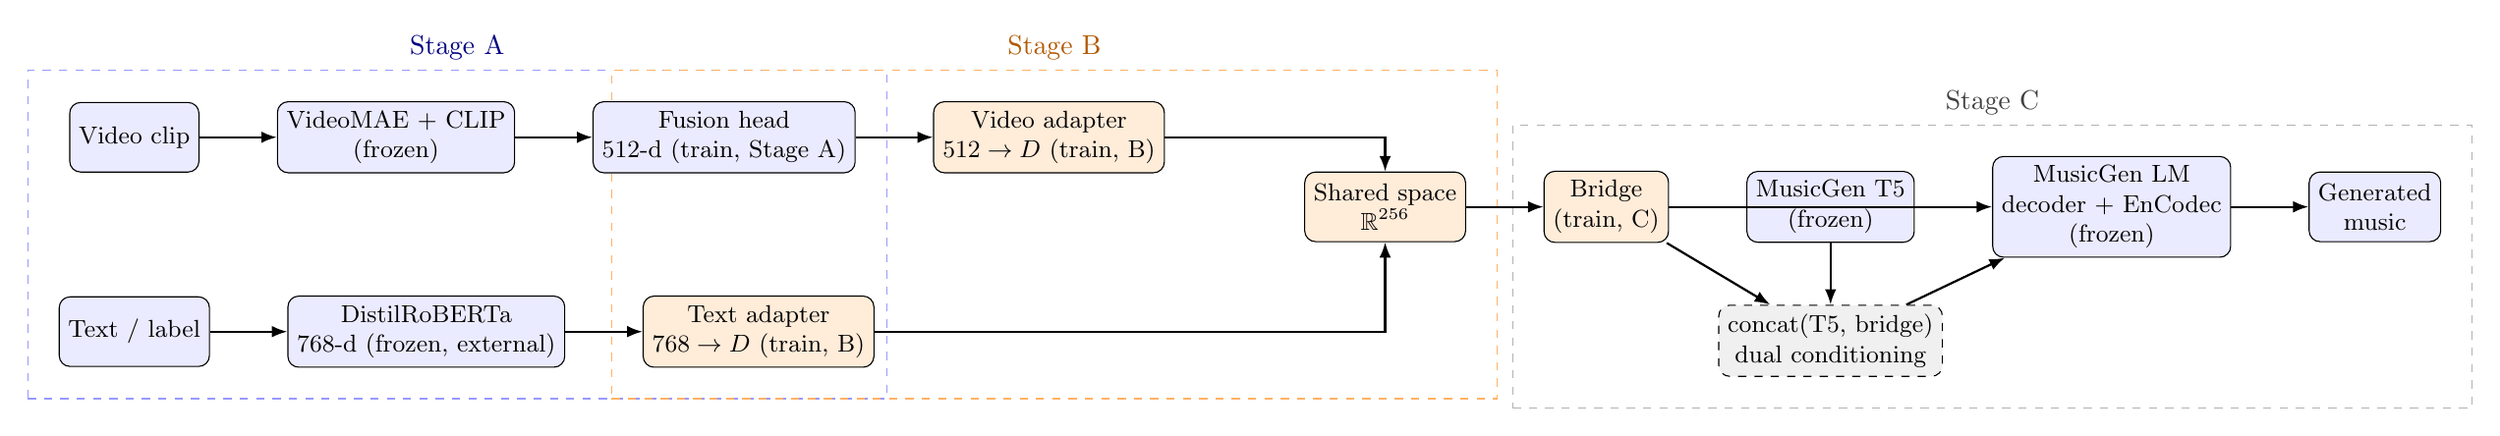
\begin{tikzpicture}[
  node distance=8mm and 10mm,
  box/.style={rectangle, draw, rounded corners, minimum height=9mm, align=center, font=\small},
  frozen/.style={box, fill=blue!8},
  train/.style={box, fill=orange!15},
  future/.style={box, fill=gray!12, dashed},
  arr/.style={-{Latex[length=2mm]}, thick}
]
\node[frozen] (vid) {Video clip};
\node[frozen, right=of vid] (vmae) {VideoMAE + CLIP\\(frozen)};
\node[frozen, right=of vmae] (vhead) {Fusion head\\512-d (train, Stage A)};
\node[train, right=of vhead] (vadapt) {Video adapter\\$512\to D$ (train, B)};

\node[frozen, below=16mm of vid] (txt) {Text / label};
\node[frozen, right=of txt] (roberta) {DistilRoBERTa\\768-d (frozen, external)};
\node[train, right=of roberta] (tadapt) {Text adapter\\$768\to D$ (train, B)};

\node[train, right=18mm of vadapt, yshift=-9mm] (shared) {Shared space\\$\mathbb{R}^{256}$};

\node[train, right=of shared] (bridge) {Bridge\\(train, C)};
\node[frozen, right=of bridge] (t5) {MusicGen T5\\(frozen)};
\node[future, below=8mm of t5] (concat) {concat(T5, bridge)\\dual conditioning};
\node[frozen, right=of t5] (musicgen) {MusicGen LM\\decoder + EnCodec\\(frozen)};
\node[frozen, right=of musicgen] (music) {Generated\\music};

\draw[arr] (vid) -- (vmae);
\draw[arr] (vmae) -- (vhead);
\draw[arr] (vhead) -- (vadapt);
\draw[arr] (txt) -- (roberta);
\draw[arr] (roberta) -- (tadapt);
\draw[arr] (vadapt.east) -| (shared.north);
\draw[arr] (tadapt.east) -| (shared.south);
\draw[arr] (shared) -- (bridge);
\draw[arr] (bridge) -- (concat);
\draw[arr] (t5) -- (concat);
\draw[arr] (concat) -- (musicgen);
\draw[arr] (bridge) -- (musicgen);
\draw[arr] (musicgen) -- (music);

\begin{scope}[on background layer]
\node[fit=(vid)(vmae)(vhead)(txt)(roberta), draw=blue!40, dashed, inner sep=4mm,
  label={[blue!50!black]above:Stage A}] {};
\node[fit=(vadapt)(tadapt)(shared), draw=orange!60, dashed, inner sep=4mm,
  label={[orange!70!black]above:Stage B}] {};
\node[fit=(bridge)(t5)(concat)(musicgen)(music), draw=gray!60, dashed, inner sep=4mm,
  label={[gray!50!black]above:Stage C}] {};
\end{scope}
\end{tikzpicture}%
}
\end{center}
\captionof{figure}{Full pipeline. Blue = frozen pretrained component. Orange = trained in this
project. The dual-conditioning concatenation path (Section~\ref{sec:dual}) is an extension of the
original single-source bridge design.}
\label{fig:pipeline}

\section{Dataset and Preprocessing}
\label{sec:data}

\subsection{Raw data}
The project builds on the EmoMV dataset, distributed as three sub-collections (DS1, DS2, DS3),
each with a headerless 7-column annotation CSV per split giving a clip's relative directory, file
stem, a \texttt{match\_lbl} flag, and an emotion label. \texttt{match\_lbl} distinguishes
\emph{MATCH} rows (video content and the labeled emotion agree by the dataset's own construction)
from \emph{MISMATCH} rows (deliberately paired with a different, non-corresponding emotion, used
in the original EmoMV benchmark for retrieval-style tasks). An exploratory data analysis
(\texttt{emomv\_eda.ipynb}, \texttt{eda\_outputs/eda\_summary.json}) preceded pipeline construction
and reported: 6{,}452 physical \texttt{.mp4} files on disk, 0 corrupt/unreadable files, 0
annotation entries missing on disk, 3{,}178 MATCH pairs and 2{,}808 MISMATCH pairs, dominant
resolution 640$\times$360 (16:9, landscape), dominant FPS 25.0, dominant codec h264, and a median
file size of 2.20\,MB (15.89\,GB on disk in total). The EDA also ran pairwise two-sample
Kolmogorov--Smirnov tests on clip-duration distributions across DS1/DS2/DS3 and found
statistically significant differences among all three sub-datasets --- i.e., a real domain shift,
not just a labeling artifact --- which is the reason every downstream evaluation in this project
is reported broken out per dataset source rather than only pooled (Section~\ref{sec:eval}).

\subsection{Manifest construction (Phase 1)}
\label{sec:manifest}
\texttt{project/preprocessing/build\_manifest.py} is the single source of truth every later phase
reads from. Its pipeline, in order:
\begin{enumerate}
  \item \textbf{Parse annotations, MATCH-only.} Only rows with \texttt{match\_lbl == 1} are kept
  (config key \texttt{match\_lbl\_keep: 1}) --- MISMATCH rows are dropped entirely to avoid label
  ambiguity/leakage in a mood-classification setting.
  \item \textbf{Emotion normalization.} Raw emotion strings are lower-cased and passed through an
  alias table (\texttt{emotion\_aliases} in \texttt{config.yaml}: \texttt{happy}$\to$\texttt{exciting},
  \texttt{excitement}$\to$\texttt{exciting}, \texttt{contentment}$\to$\texttt{relax},
  \texttt{relaxing}$\to$\texttt{relax}, \texttt{fearful}$\to$\texttt{fear},
  \texttt{tension}$\to$\texttt{tense}) before being mapped to one of 5 integer class ids
  (\texttt{exciting=0, fear=1, tense=2, sad=3, relax=4}).
  \item \textbf{Drop missing files.} Any annotation row whose referenced \texttt{.mp4} is absent on
  disk is dropped.
  \item \textbf{Container probing.} Every remaining file is opened with OpenCV to confirm it is
  decodable and to record FPS, frame count, and duration; unreadable clips are dropped.
  \item \textbf{Exact deduplication.} Every clip is SHA-256 hashed; clips with identical hashes are
  exact duplicates and only the first-seen copy is kept. This step found \textbf{34 duplicate
  pairs}, of which \textbf{2 pairs had conflicting emotion labels} (the same physical video
  annotated with two different moods across sub-datasets) --- these conflicts are resolved by
  keeping the first-seen annotation, and are logged to
  \texttt{project/data/duplicates\_report.csv} for manual inspection rather than silently
  discarded.
  \item \textbf{Group-id derivation.} A \texttt{source\_group\_id} is derived per clip so that
  segments of the same underlying source video are never split across train/val/test
  (Section~\ref{sec:split}): DS1 stems of the form \texttt{..\_name-2-of-8.mp4} have the
  \texttt{-\textit{k}-of-\textit{n}} suffix stripped via regex; DS3 stems of the form
  \texttt{<youtube\_id>\_02.mp4} have the trailing 2-digit segment index stripped; DS2 stems are
  used as-is (bare YouTube ids, no observed segmentation).
  \item \textbf{Duration-outlier windowing.} Clips whose duration exceeds
  \texttt{max\_duration\_s + tolerance\_s} $= 30+5=35$\,s are treated as genuine outliers (not the
  much larger set of clips that merely round to 30.0--30.5\,s from encoding) --- \textbf{20 such
  outliers} were found (mean duration 87.9\,s, max 392.4\,s), logged to
  \texttt{project/data/duration\_outliers.csv}, and split into non-overlapping
  \texttt{window\_s}$=30$\,s windows (\texttt{project/preprocessing/duration\_windows.py}); a
  trailing remainder shorter than \texttt{min\_window\_remainder\_s}$=5$\,s is dropped rather than
  kept as an undersized window. No video is re-encoded --- only \texttt{(start\_frame,
  end\_frame)} ranges are computed; the dataset class slices lazily at decode time.
\end{enumerate}

\paragraph{Resulting manifest.} The final manifest (\texttt{project/data/manifest.csv}) contains
\textbf{3{,}189 rows} (windowed sub-clips included) covering \textbf{3{,}144 unique parent
videos}. Per-dataset-source counts: DS1 = 2{,}653, DS2 = 308, DS3 = 228. Per-emotion counts:
exciting = 689, fear = 537, tense = 459, sad = 594, relax = 910 (a roughly 2:1 imbalance between
the largest and smallest class).

\subsection{Train/val/test split (Phase 2)}
\label{sec:split}
\texttt{project/preprocessing/split.py} rebuilds the train/val/test assignment from scratch rather
than using EmoMV's own official split, because the official split was found to leak: clips
segmented from the same source video (the \texttt{-\textit{k}-of-\textit{n}} DS1 naming
convention) land in different splits under it --- 37 groups span train/val, 23 span train/test,
and 34 span val/test in the official assignment. The replacement algorithm is a \textbf{greedy
iterative stratification}: \texttt{source\_group\_id} groups are shuffled deterministically (seed
42), then each group is assigned, one at a time, to whichever split currently has the largest
\emph{deficit} against its target fraction for that group's (majority) emotion class. This gives
precise 70/15/15 control (\texttt{train\_frac}$=0.70$, \texttt{val\_frac}$=0.15$,
\texttt{test\_frac}$=0.15$) while guaranteeing zero cross-split group leakage by construction ---
verified post-hoc by an assertion that no \texttt{source\_group\_id} has more than one unique split
value. The resulting split sizes, broken out per dataset source, are:
\begin{center}
\begin{tabular}{@{}lrrrr@{}}
\toprule
Split & Rows & DS1 & DS2 & DS3 \\
\midrule
train & 2{,}232 & 1{,}870 & 190 & 172 \\
val & 479 & 395 & 59 & 25 \\
test & 478 & 388 & 59 & 31 \\
\bottomrule
\end{tabular}
\end{center}
DS1 dominates at 83\% of all clips, a fact worth keeping in mind when reading the per-dataset
results in Section~\ref{sec:results}. Class-imbalance weighting (Section~\ref{sec:train-stageA})
uses inverse-frequency weights derived from the training-set class counts; the EDA's own
precomputed reference values were exciting~0.858, fear~1.104, tense~1.321, sad~1.084, relax~0.800
(imbalance ratio $\approx1.65\times$ between the most- and least-frequent class).

\subsection{Video decoding and frame sampling (Phase 3)}
\texttt{project/datasets/video\_dataset.py}'s \texttt{EmoMVVideoDataset} turns a manifest row into
a $(T,C,H,W)$ tensor of frames in $[0,1]$ (per-encoder normalization is applied later, in
\texttt{models/encoders.py}, so the same decoded clip can feed both frozen encoders without
re-decoding). $T=16$ frames (\texttt{num\_frames}) are sampled by dividing the clip's
\texttt{[start\_frame, end\_frame)} range into 16 equal segments; in \texttt{mode="train"} a
uniformly random position within each segment is sampled (temporal jitter), while in
\texttt{mode="val"/"test"} the deterministic segment midpoint is used, so validation/test
embeddings are reproducible across runs. Frames are then resized so the shorter edge is 256\,px
and center-cropped to $224\times224$ (\texttt{resize\_shorter\_edge}, \texttt{crop\_size}), then
converted BGR$\to$RGB. Decode failures are handled per-frame (a failed frame is zero-padded, logged
via a dedicated logger to \texttt{project/logs/dataset\_errors.log}) rather than failing the whole
batch. Feature extraction (Phase 4) always uses \texttt{mode="val"} deterministic sampling, even
for the training split, since embeddings are computed once and cached rather than resampled every
epoch.

\subsection{Frozen encoder feature extraction (Phase 4)}
\texttt{project/features/extract\_features.py} runs two frozen HuggingFace encoders over every
manifest row and caches one tensor per clip per encoder (skipping any clip whose cache file
already exists, so re-running is idempotent):
\begin{itemize}
  \item \textbf{VideoMAE} (\texttt{MCG-NJU/videomae-base}): frames are normalized with VideoMAE's
  own per-channel mean/std, passed through the frozen model, and the \texttt{last\_hidden\_state}
  is mean-pooled over the token/time dimension to a \textbf{768-d} vector.
  \item \textbf{CLIP} (\texttt{openai/clip-vit-base-patch32}): each of the 16 frames is
  individually normalized with CLIP's own mean/std, passed through
  \texttt{get\_image\_features}, and the resulting per-frame 512-d embeddings are mean-pooled over
  the 16 frames to a \textbf{512-d} vector.
\end{itemize}
Both encoders are wrapped with \texttt{requires\_grad=False} on every parameter and run under
\texttt{torch.no\_grad()} at all times; extraction uses batch size 8
(\texttt{encoders.batch\_size}) with device preference \texttt{["mps","cuda","cpu"]}.

\subsection{SlowFast baseline features}
As a reference point that requires no new video decoding, \texttt{project/features/}
\texttt{extract\_slowfast\_baseline.py} re-aligns the dataset's own shipped, pre-extracted SlowFast
features (\texttt{.h5} files, one row per line of the \emph{original} MATCH+MISMATCH annotation
CSV, in the same row order --- verified directly by comparing row counts) with the MATCH-only
manifest, keeping only \texttt{match\_lbl==1} rows and caching each as a
\texttt{features/slowfast/<parent\_video\_id>.pt} (2{,}304-d). SlowFast features exist only per
whole original clip, not per window, so a windowed manifest row is keyed by its
\texttt{parent\_video\_id} rather than its own \texttt{video\_id} when loaded
(\texttt{CachedEmbeddingDataset}'s \texttt{key\_column} argument handles this distinction
generically).

\subsection{Text mood classifier (external asset)}
\label{sec:text-encoder}
The text-side mood classifier (\texttt{project/text\_mood\_clf\_encoder/text\_mood\_clf}) is a
\textbf{pretrained, externally fine-tuned} \texttt{distilroberta-base}
(\texttt{RobertaForSequenceClassification}; 6 transformer layers, hidden size 768, 12 attention
heads, vocab 50{,}265) reporting test macro-F1 $\approx 0.80$ on the same 5-class label set
(labels: \texttt{excited, fear, tense, sad, relax} --- identical ordering to the video side except
for the ``exciting'' vs.\ ``excited'' lexical difference, which is a deliberate, useful coincidence
that avoids needing a label-id remapping table between the two modalities). Unlike the video
fusion head, this is a genuine end-to-end fine-tune: RoBERTa's own backbone weights were updated
during its (external) training, not just a linear head on top of frozen features. This project
consumes it purely as a frozen encoder (\texttt{FrozenTextMoodEncoder} in
\texttt{project/models/encoders.py}), exposing its \textbf{768-d penultimate representation}
(post dense$+$tanh, pre \texttt{out\_proj}) rather than its final logits, by manually replaying
\texttt{roberta} $\to$ \texttt{classifier.dropout} $\to$ \texttt{classifier.dense} $\to$
\texttt{tanh} $\to$ \texttt{classifier.dropout}. This reconstruction was verified to reproduce the
model's own \texttt{.logits} output exactly before being relied upon, and is symmetric to how
\texttt{FusionClassifier}'s own penultimate 512-d layer is used on the video side
(Section~\ref{sec:embedding-choice}).

\subsection{512-d task-supervised video embedding caching}
Once the Stage A fusion classifier is trained (Section~\ref{sec:stageA-video}),
\texttt{project/features/extract\_video\_embedding\_512.py} caches its 512-d \emph{penultimate}
activation (everything in \texttt{FusionClassifier} except the final \texttt{Linear(512,5)}) for
every clip to \texttt{features/video\_embedding\_512/<video\_id>.pt}. This --- not the raw
1280-d VideoMAE+CLIP concatenation, and not the 5-class logits --- is the representation Stage B's
video adapter projects from (Section~\ref{sec:embedding-choice}).

\subsection{Audio target extraction for Stage C}
\texttt{project/features/extract\_audio\_targets.py} extracts each MATCH clip's own audio track
via \texttt{ffmpeg} (\texttt{-vn -ac \{channels\} -ar \{sample\_rate\}}), respecting a windowed
sub-clip's \texttt{(start\_frame, end\_frame)} boundaries by converting them to \texttt{-ss}/\texttt{-t}
seconds via the clip's own FPS. Output is resampled to \textbf{32\,kHz mono} --- the input format
MusicGen-small's EnCodec tokenizer expects (\texttt{stage\_c.audio\_sample\_rate=32000},
\texttt{audio\_channels=1}). This is a deliberate reuse of an existing resource: since EmoMV's
MATCH clips have video emotion equal to music emotion \emph{by the dataset's own construction},
every one of these clips' own soundtracks is already a mood-consistent generation target, requiring
no new data collection --- only extraction. Two caveats are documented but \emph{not} acted upon in
this project (Section~\ref{sec:experiments}): the extracted audio is a music-video soundtrack that
may contain vocals, sound effects, or dialogue rather than a clean instrumental bed, and it is used
as-is.

\section{Model Architectures}
\label{sec:models}

\subsection{Stage A: baseline classifier (\texttt{SlowFastBaselineMLP})}
A simple reference classifier over the shipped, pre-extracted SlowFast features, established
before investing in the frozen VideoMAE+CLIP fusion model:
\[
\mathbb{R}^{2304} \xrightarrow{\text{Linear}} \mathbb{R}^{256} \xrightarrow{\text{ReLU, Dropout}(0.3)} \mathbb{R}^{256} \xrightarrow{\text{Linear}} \mathbb{R}^{5}.
\]

\subsection{Stage A: video fusion classifier (\texttt{FusionClassifier})}
\label{sec:stageA-video}
Concatenates the frozen VideoMAE (768-d) and CLIP (512-d) embeddings (Section~\ref{sec:data}) into
a 1280-d vector and classifies it with a single hidden layer:
\[
\mathbb{R}^{1280} \xrightarrow{\text{Linear}} \mathbb{R}^{512} \xrightarrow{\text{GELU, Dropout}(0.3)} \mathbb{R}^{512} \xrightarrow{\text{Linear}} \mathbb{R}^{5}.
\]
The forward pass supports a \texttt{return\_embedding=True} flag that returns the 512-d activation
\emph{after} GELU+Dropout but \emph{before} the final \texttt{Linear(512,5)} --- indexing directly
into the underlying \texttt{nn.Sequential} rather than restructuring the module, so an already
trained checkpoint's \texttt{state\_dict} layout is unaffected. Only VideoMAE and CLIP's own
weights are frozen here; this fusion head itself is trained from scratch (Section~\ref{sec:train-stageA}).

\subsection{Stage B: cross-modal alignment (\texttt{AlignmentModel})}
\label{sec:stageB-model}
Two structurally symmetric MLP adapters project each modality's frozen, task-supervised
penultimate embedding into a shared $D=256$-dimensional space:
\[
\text{video\_adapter}: \mathbb{R}^{512}\to\mathbb{R}^{256}, \qquad
\text{text\_adapter}: \mathbb{R}^{768}\to\mathbb{R}^{256},
\]
each implemented identically apart from input width as
\[
\text{Linear}(d_{\text{in}}, 2D) \to \text{LayerNorm} \to \text{GELU} \to \text{Dropout}(0.15) \to \text{Linear}(2D, D),
\]
followed by L2 normalization $\hat z = z/\lVert z\rVert_2$ so downstream similarities are pure
cosine similarities (the same convention CLIP uses). A learnable temperature
(\texttt{LogitScale}) is parameterized in log-space as CLIP does,
$\text{logit\_scale}=\exp(\min(\log s, \log s_{\max}))$, initialized at $s=1/0.07\approx14.2857$
and clamped to a maximum of $100$. \texttt{AlignmentModel} bundles both adapters and the
temperature into a single checkpointable module with \texttt{encode\_video}/\texttt{encode\_text}
methods.

\subsubsection{Which embedding is projected, and why}
\label{sec:embedding-choice}
Stage B deliberately does \emph{not} project the raw 1280-d VideoMAE+CLIP concatenation or
RoBERTa's raw token embeddings. It projects the \emph{penultimate, task-supervised} representation
from each existing Stage A classifier (Section~\ref{sec:stageA-video}, Section~\ref{sec:text-encoder}).
Both are already the result of supervised training toward the same 5-class taxonomy, so the
adapters only need to learn a geometric alignment of two already-discriminative spaces, rather than
starting from generic, task-agnostic backbone features.

\subsection{Stage C: bridge network (\texttt{EmbeddingToConditioningBridge})}
\label{sec:bridge-model}
MusicGen does not consume a single conditioning vector; its cross-attention expects a
\emph{sequence} of $(T,768)$ hidden states (T5's hidden size), the same shape its own frozen T5
text encoder would normally produce for a text prompt. The bridge's job is to turn Stage B's single
256-d point $z$ into such a sequence:
\begin{enumerate}
  \item \textbf{Input projection.} $z\in\mathbb{R}^{256}$ is linearly projected to
  $\mathbb{R}^{512}$ (\texttt{hidden\_dim}) and treated as a single ``memory'' token,
  $(B,1,512)$.
  \item \textbf{Learned queries.} A learned parameter tensor of shape $(8,512)$
  (\texttt{seq\_len}=8, initialized $\mathcal{N}(0,0.02^2)$) is broadcast across the batch as the
  target sequence for a standard \texttt{nn.TransformerDecoder} (2 layers, 4 heads,
  feed-forward dim $=2\times512=1024$, dropout 0.1, batch-first). Each decoder layer lets the 8
  queries self-attend among themselves and cross-attend to the single memory token.
  \item \textbf{Output projection.} The decoded $(B,8,512)$ sequence is linearly projected to
  $\mathbb{R}^{768}$ (MusicGen's T5 hidden size) and passed through a final \texttt{LayerNorm}.
\end{enumerate}
The bridge always emits a fixed-length, unpadded 8-token sequence, so its accompanying attention
mask is simply all-ones. Only this bridge network is ever trained in Stage C
(Section~\ref{sec:train-stageC}); everything upstream (Stage A/B) and downstream (MusicGen) is
frozen.

\subsection{MusicGen (frozen generative backbone)}
The generator is \texttt{facebook/musicgen-small} via
\texttt{transformers.MusicgenForConditionalGeneration}: an autoregressive transformer over
discrete EnCodec audio tokens, text-conditioned via a T5 encoder whose hidden-state sequence is
cross-attended by every decoder layer. All of MusicGen's parameters --- the T5 text encoder, the
EnCodec tokenizer/decoder, and the LM decoder itself --- are frozen throughout this project
(\texttt{requires\_grad=False} on every parameter, model kept in \texttt{.eval()}). Verified
directly against the installed \texttt{transformers} source
(\texttt{modeling\_musicgen.py}): if \texttt{encoder\_outputs} is not supplied to
\texttt{.forward()}/\texttt{.generate()}, MusicGen calls its own T5 encoder on \texttt{input\_ids};
if it \emph{is} supplied (as a tuple), it is wrapped directly into a \texttt{BaseModelOutput} and
used as-is, regardless of its source or sequence length --- this is the hook both the single-source
bridge and the dual-conditioning extension exploit. A config-loading quirk in the installed
\texttt{transformers} version is fixed defensively in both training scripts:
\texttt{musicgen.config.decoder.decoder\_start\_token\_id} loads as \texttt{None} even though
\texttt{generation\_config.decoder\_start\_token\_id} (the reserved EnCodec pad token, 2048) is set
correctly, and is copied over before training since \texttt{shift\_tokens\_right} needs it.

\subsection{Dual-conditioning module (\texttt{project/models/conditioning.py})}
\label{sec:dual-model}
A small set of stateless helpers supporting the concatenated-conditioning extension
(Section~\ref{sec:dual}):
\begin{itemize}
  \item \texttt{build\_musicgen\_tokenizer}: loads the T5 tokenizer shipped with the MusicGen
  checkpoint (the same tokenizer stock MusicGen uses internally).
  \item \texttt{t5\_encode}: runs raw text through MusicGen's own frozen
  \texttt{musicgen.text\_encoder} under \texttt{no\_grad}, returning \emph{both} the hidden-state
  sequence $(B,T_{\text{text}},768)$ and its padding mask --- exactly what stock MusicGen computes
  internally for a text prompt, just exposed for reuse.
  \item \texttt{concat\_conditioning}: concatenates the T5 sequence and the bridge's sequence along
  the time axis, and concatenates their masks correspondingly:
  \[
  \text{cond} = [\,T5(\text{text})\,;\,\text{bridge}(z)\,] \in \mathbb{R}^{B\times(T_{\text{text}}+T_{\text{bridge}})\times768},
  \qquad
  \text{mask} = [\,\text{mask}_{T5}\,;\,\mathbf{1}_{T_{\text{bridge}}}\,].
  \]
  \item \texttt{label\_template\_text}: builds the raw-text input for a clip from its integer
  emotion label via a fixed template (e.g.\ \texttt{"\{emotion\} instrumental music"} $+$ label 4
  $\to$ \texttt{"relax instrumental music"}), since EmoMV clips carry no per-clip captions.
\end{itemize}

\section{Training Methodology}
\label{sec:training}

\subsection{Stage A: classifier training}
\label{sec:train-stageA}
Both the SlowFast-baseline MLP and the VideoMAE+CLIP fusion classifier share one training loop
(\texttt{project/training/loop.py}, \texttt{train\_classifier}):
\begin{itemize}
  \item \textbf{Optimizer:} \texttt{torch.optim.Adam}, learning rate $3\times10^{-4}$, weight decay
  $10^{-4}$ (\texttt{training.lr}, \texttt{training.weight\_decay}).
  \item \textbf{Batching:} batch size 32, 4 dataloader workers.
  \item \textbf{Class imbalance:} \texttt{class\_imbalance\_strategy} supports two interchangeable
  options, selected via config (Section~\ref{sec:experiments}): \texttt{"class\_weights"} (inverse-frequency
  weights $w_k = N/(K\cdot n_k)$ fed into a weighted \texttt{nn.CrossEntropyLoss}) --- the option
  actually used for all reported runs --- or \texttt{"weighted\_sampler"} (a
  \texttt{WeightedRandomSampler} built from the same per-class weights).
  \item \textbf{Early stopping:} patience 10 epochs, monitored on validation macro-F1 (maximize),
  up to 100 epochs.
  \item \textbf{Checkpointing:} the best-macro-F1 epoch's model/optimizer state is saved to
  \texttt{fusion\_classifier\_best.pt} / \texttt{baseline\_slowfast\_mlp\_best.pt}.
\end{itemize}
The fusion classifier uses \texttt{fusion\_hidden\_dim}=512, \texttt{fusion\_dropout}=0.3; the
baseline uses \texttt{baseline\_hidden\_dim}=256, \texttt{baseline\_dropout}=0.3. In the recorded
run, the SlowFast baseline early-stopped at \textbf{epoch 44} (best validation macro-F1 0.525)
while the fusion classifier converged far faster, early-stopping by \textbf{epoch 10} (best
validation macro-F1 0.807) --- frozen VideoMAE/CLIP embeddings evidently carry substantially more
emotion-discriminative signal than the shipped SlowFast features even into an identically-sized MLP
head. Validation and test macro-F1 for the fusion model are close (0.807 vs.\ 0.794), giving no
strong indication of overfitting to the validation split.

\subsection{Stage B: label-anchored contrastive alignment training}
\label{sec:train-stageB}
\texttt{project/training/train\_alignment.py} trains only the two Stage B adapters and the
temperature (Section~\ref{sec:stageB-model}); the frozen encoders that produced the cached
embeddings are never touched.

\paragraph{The pairing problem.} Standard CLIP-style contrastive training assumes naturally
occurring (image, caption) instance pairs. This project has no such pairs --- only $\sim$3{,}144
videos and a text corpus, each independently carrying one of the same 5 categorical mood labels,
with no instance-level video$\leftrightarrow$sentence correspondence. Rather than collect or
synthesize pairs, Stage B uses exactly \textbf{5 fixed text anchors} --- the 5 class-name strings
themselves (\texttt{load\_text\_anchors} in \texttt{project/training/alignment\_common.py}), each
encoded once through the frozen text encoder into a $(5,768)$ tensor. This is documented in the
code as a deliberate, honest simplification (no larger text training corpus was available), not an
oversight.

\paragraph{Loss (\texttt{project/training/losses.py}).} With the text side reduced to 5 fixed
anchors, the video$\to$text direction is a plain 5-way softmax cross-entropy (mathematically
InfoNCE with the 4 other anchors as in-batch negatives):
\[
\mathcal{L}_{\text{v2t}} = -\frac{1}{N}\sum_i \log\frac{\exp(s_{i,y_i})}{\sum_{c=1}^{5}\exp(s_{ic})},
\qquad s_{ic} = \text{logit\_scale}\cdot \hat v_i\cdot \hat t_c.
\]
The text$\to$video direction is the multi-positive supervised-contrastive generalization (Khosla et
al., 2020), since many videos in a batch can share a given anchor's class:
\[
\mathcal{L}_i = -\frac{1}{|P(i)|}\sum_{p\in P(i)}\log\frac{\exp(s_{ip})}{\sum_a \exp(s_{ia})},
\qquad P(i) = \{\text{videos in-batch sharing anchor } i\text{'s class}\}.
\]
The total loss is the mean of the two directions, $\mathcal{L}=\tfrac12(\mathcal{L}_{\text{v2t}}+\mathcal{L}_{\text{t2v}})$.
No auxiliary classification loss term is present in the implemented loss function (one was
proposed in the planning document as a safeguard against representation collapse, but the shipped
\texttt{label\_anchored\_contrastive\_loss} implements only the contrastive terms above ---
Section~\ref{sec:experiments}).

\paragraph{Optimization.} AdamW, learning rate $10^{-3}$, weight decay $10^{-4}$, batch size 128,
up to 200 epochs, early stopping patience 15 epochs on validation video$\to$text accuracy
(maximize). \texttt{shared\_dim}=256, \texttt{adapter\_dropout}=0.15. Because there are exactly 5
fixed text anchors, video$\to$text Recall@1 collapses to simple 5-way classification accuracy
against the anchors as class prototypes --- this identity is used directly as the monitored/early-stopping metric. The recorded run early-stopped at \textbf{epoch 25}, with a best
\emph{validation} video$\to$text accuracy of \textbf{0.8205}; the \emph{held-out test} accuracy
reported in Section~\ref{sec:results} (0.8096) is evaluated separately, after training, on the test
split the early-stopping criterion never saw.

\subsection{Stage C, Milestone 1: single-source bridge training}
\label{sec:train-stageC}
\texttt{project/training/train\_bridge.py} pairs each clip's cached 512-d video embedding with its
own extracted audio waveform (\texttt{VideoEmbeddingAudioDataset}) --- no additional pairing effort
is needed, since a MATCH clip's video and audio are already the same underlying file. Waveforms are
truncated/zero-padded to \texttt{clip\_duration\_s}=10\,s at 32\,kHz.

\paragraph{Objective.} MusicGen's own teacher-forced next-token cross-entropy loss over EnCodec
audio codes --- the same objective MusicGen's text-conditioning pathway was originally trained
with; only the conditioning \emph{source} changes. The target waveform is encoded to EnCodec codes
via \texttt{musicgen.audio\_encoder.encode} (asserting exactly one EnCodec frame, i.e.\ chunking
disabled) and reshaped to the \texttt{(B, seq\_len, num\_codebooks)} layout
\texttt{MusicgenForConditionalGeneration.forward} expects for its \texttt{labels} argument (distinct
from the \texttt{(B*num\_codebooks, seq\_len)} layout used for \texttt{input\_ids}). Each step:
$z=\texttt{alignment\_model.encode\_video}(\text{video\_emb})$ (frozen, no grad)
$\to$ $\text{cond}=\text{bridge}(z)$ (only tensor with gradients) $\to$
\texttt{musicgen(encoder\_outputs=(cond,), attention\_mask=..., labels=codec\_labels)}.

\paragraph{Optimization.} AdamW on \texttt{bridge.parameters()} only, learning rate $3\times10^{-4}$,
weight decay $10^{-5}$, batch size 4, early stopping patience 5 (minimize validation loss). The
\emph{originally committed} configuration ran this as a deliberately small-scale sanity check ---
\texttt{subset\_size}=300 training clips (validation subset $=\max(300/5,10)=60$), \texttt{max\_epochs}=2
--- consistent with the planning document's recommendation to validate cheaply that the shared
space carries usable conditioning signal at all before scaling up. The checkpoint from this run is
\texttt{bridge\_best.pt}.

\subsection{Stage C extension: dual conditioning}
\label{sec:dual}
A later, currently-uncommitted round of work (config changes and a new
\texttt{project/models/conditioning.py} module, both present in the working tree but not yet
merged into version control at the time of this report) extends Milestone 1 as proposed in
\texttt{project/docs/text\_conditioning\_bridge\_plan.pdf}: rather than the bridge output
\emph{replacing} MusicGen's T5 conditioning outright, MusicGen's own frozen T5 encoder is run on
raw text (a per-clip templated string, Section~\ref{sec:dual-model}, since no real per-clip
captions exist) and its output is \textbf{concatenated} with the bridge's mood-steering sequence
before cross-attention (Section~\ref{sec:dual-model}). The motivation: the original design gives
MusicGen \emph{only} the collapsed 5-class mood point as its entire conditioning input, discarding
any richer descriptive content (instrumentation, genre, tempo) that raw text could carry.

\paragraph{What changed mechanically.} \texttt{train\_bridge.py}'s dataset and training loop gained
a \texttt{dual\_conditioning} branch (config flag \texttt{stage\_c.dual\_conditioning: true}): each
batch's raw text is built from its integer label via \texttt{label\_template\_text} with template
\texttt{"\{emotion\} instrumental music"} (\texttt{text\_template}, max length 64 tokens), encoded
through the frozen T5 (\texttt{t5\_encode}, no gradient), and concatenated with the bridge's own
output (\texttt{concat\_conditioning}) before being passed to MusicGen. \textbf{Only the bridge
still receives gradients} --- T5 is run under \texttt{no\_grad} either way, so this adds no
optimizer state relative to Milestone 1. Because the old \texttt{bridge\_best.pt} checkpoint was
trained assuming its output was the \emph{sole} conditioning source, it is not reused as-is: a
separate checkpoint name, \texttt{bridge\_dual\_best.pt} (\texttt{bridge\_checkpoint\_name} config
key), keeps the two trainings independent so the original bridge-only baseline remains available
for comparison. A \texttt{resume: true} config flag was also added, allowing training to reload an
existing checkpoint (model, optimizer state, epoch counter, and best validation score) and continue
rather than restart from scratch. Alongside this, \texttt{max\_epochs} was raised from 2 to 200 and
\texttt{subset\_size} from 300 to 9{,}999 (i.e.\ effectively uncapped, using the entire available
train/val pool with cached audio) for this extended run. A \texttt{bridge\_dual\_best.pt} checkpoint
exists in \texttt{project/training/checkpoints/}, confirming this training was actually executed
(not merely planned).

\subsection{Notebook-driven training}
Every training script above has a parallel, cell-by-cell notebook counterpart intended for
interactive runs with live progress bars and inline audio playback rather than being invoked as a
background process: \texttt{05\_train.ipynb} (Stage A), \texttt{07\_alignment.ipynb} (Stage B), and
\texttt{08\_bridge.ipynb} (Stage C, updated in place to add the dual-conditioning path and its
three-way generation/ablation cells, Section~\ref{sec:eval-stageC}).

\section{Evaluation Methodology}
\label{sec:eval}

\subsection{Stage A: classifier evaluation}
\texttt{project/evaluation/evaluate.py} loads a trained checkpoint (baseline or fusion), predicts
over the held-out test split, and reports accuracy, macro-F1, and weighted-F1 both \textbf{overall}
and broken out \textbf{per dataset source (DS1/DS2/DS3)} --- the per-dataset breakdown exists
specifically because the EDA's confirmed domain shift (Section~\ref{sec:data}) means a model that
only fits DS1 should show up as a DS2/DS3 gap in this report, not just a mediocre pooled number.
Confusion matrices are rendered and saved per breakdown (\texttt{*\_confusion\_matrix\_\{overall,DS1,DS2,DS3\}.png})
alongside a JSON metrics dump.

\subsection{Stage B: alignment evaluation}
\texttt{project/evaluation/evaluate\_alignment.py} reports, again overall and per dataset source:
\begin{itemize}
  \item \textbf{Video$\to$text accuracy / Recall@1}: with only 5 fixed anchors, this is exactly
  5-way classification accuracy using the anchors as class prototypes (nearest anchor by cosine
  similarity). Text$\to$video retrieval is explicitly \emph{not} reported --- with no diversity on
  the text side, there is nothing meaningful to retrieve \emph{among} on that side, and the code
  comments document this omission rather than silently reporting only the flattering half.
  \item \textbf{Per-class recall.}
  \item \textbf{Modality-gap diagnostic}: for each class, the cosine similarity between that
  class's video-embedding centroid and its text anchor --- CLIP-family models are documented to
  retain a persistent ``modality gap'' (the two modalities occupying separate sub-manifolds even
  after contrastive training), so this is measured explicitly rather than assumed away.
  \item \textbf{Qualitative t-SNE plot} of the shared space (video points colored/shaped by class,
  text anchors shown as large stars), to visually check that same-label points from both
  modalities cluster together rather than forming two same-colored but separate modality islands.
\end{itemize}

\subsection{Stage C: qualitative generation evaluation}
\label{sec:eval-stageC}
Stage C has \textbf{no automatic acoustic metric} (e.g.\ no Fr\'echet Audio Distance or CLAP score
is computed anywhere in the codebase) --- evaluation is a deliberate, documented
\emph{manual-listening} protocol via \texttt{project/evaluation/generate\_samples.py}, chosen
because the teacher-forced LM loss used for training cannot by itself distinguish ``the decoder
generates coherent audio'' from ``the decoder generates audio that reflects the requested mood.''
Samples are generated from two sources, on purpose:
\begin{enumerate}
  \item \textbf{Text anchors} (the 5 fixed class-name strings) --- out-of-distribution for the
  bridge, since it only ever trained on video embeddings; tests whether Stage B's alignment
  actually transfers to steering MusicGen from text alone.
  \item \textbf{Real video embeddings} from held-out test clips (one per emotion class) ---
  in-distribution, what the bridge was actually trained on.
\end{enumerate}
\texttt{guidance\_scale=1.0} is set explicitly in every generation call: MusicGen's default
classifier-free-guidance path duplicates the batch against an internal null/unconditional
embedding when conditioning via raw \texttt{input\_ids}, which does not apply when custom
\texttt{encoder\_outputs} are supplied directly --- disabling it avoids a shape mismatch rather than
silently producing incorrect output.

\paragraph{Three-way ablation (dual-conditioning extension).} Once dual conditioning was
implemented, sample generation was extended to produce, for every text-anchor and video-embedding
example, three variants:
\begin{itemize}
  \item \textbf{t5only}: \texttt{cond = T5(text)} alone --- the stock-MusicGen baseline the
  combined approach must beat on mood-consistency, since it is free (no training at all).
  \item \textbf{bridgeonly}: \texttt{cond = bridge(z)} alone --- the original Milestone 1 design,
  the baseline the combined approach must not regress against.
  \item \textbf{combined}: \texttt{cond = concat(T5(text), bridge(z))} --- the proposed approach.
\end{itemize}
This produced \textbf{40 output \texttt{.wav} files} in
\texttt{project/evaluation/results/generated\_samples/}: the original 10 single-source samples
(5 text-anchor + 5 video-embedding, one per class, from the Milestone-1-only
\texttt{bridge\_best.pt} run) plus 30 further samples from the three-way ablation (5 classes
$\times$ 2 sources $\times$ 3 conditioning variants, using the retrained
\texttt{bridge\_dual\_best.pt}). An \textbf{attention diagnostic} --- inspecting the decoder's
\texttt{cross\_attentions} output to check whether it collapses onto a single branch of the
concatenated sequence --- was recommended in the planning document as a cheap additional check
but was \textbf{not implemented in code}; only manual listening was actually carried out.

\section{Results}
\label{sec:results}

\subsection{Stage A: mood classification}
\begin{center}
\begin{tabular}{@{}lrrr@{}}
\toprule
Model & Accuracy & Macro-F1 & Weighted-F1 \\
\midrule
SlowFast baseline MLP (overall, $n=478$) & 50.63\% & 0.479 & 0.503 \\
\quad DS1 ($n=388$) & 54.90\% & 0.504 & 0.543 \\
\quad DS2 ($n=59$) & 33.90\% & 0.338 & 0.380 \\
\quad DS3 ($n=31$) & 29.03\% & 0.259 & 0.319 \\
\midrule
VideoMAE+CLIP fusion (overall, $n=478$) & \textbf{80.13\%} & \textbf{0.794} & \textbf{0.803} \\
\quad DS1 ($n=388$) & 86.60\% & 0.860 & 0.867 \\
\quad DS2 ($n=59$) & 52.54\% & 0.473 & 0.545 \\
\quad DS3 ($n=31$) & 51.61\% & 0.366 & 0.550 \\
\bottomrule
\end{tabular}
\end{center}
The fusion model improves substantially over the SlowFast baseline on every split, but the
DS1-vs-DS2/DS3 gap present in the baseline persists (and is not closed) in the fusion model,
consistent with the EDA's confirmed cross-dataset domain shift (Section~\ref{sec:data}) --- DS2 and
DS3 together contribute only 287 of the 3{,}189 manifest rows (9.0\%), so both models see
substantially less DS2/DS3 training signal than DS1.

\paragraph{Per-class breakdown (fusion model, overall test set).}
\begin{center}
\begin{tabular}{@{}lrrrr@{}}
\toprule
Class & Precision & Recall & F1 & Support \\
\midrule
exciting & 0.896 & 0.827 & 0.860 & 104 \\
fear & 0.655 & 0.889 & 0.754 & 81 \\
tense & 0.783 & 0.691 & 0.734 & 68 \\
sad & 0.766 & 0.809 & 0.787 & 89 \\
relax & 0.898 & 0.779 & 0.835 & 136 \\
\bottomrule
\end{tabular}
\end{center}
\texttt{tense} is the weakest class by F1; \texttt{exciting}/\texttt{relax} are strongest. The
confusion matrix shows errors clustering between \emph{adjacent} regions of the valence-arousal
plane (\texttt{tense}/\texttt{fear} are both negative-valence; \texttt{relax}/\texttt{sad} are both
low-arousal) and essentially never crossing to opposite quadrants (\texttt{exciting} is almost
never confused with \texttt{sad}) --- a positive signal that the fused embedding captures real
affective structure rather than a spurious correlation. The single largest error mode is
\texttt{tense}$\to$\texttt{fear} (25.0\% of true \texttt{tense} clips misclassified as
\texttt{fear}).

\paragraph{Small-sample caveat on the DS2/DS3 breakdown.} Part of the DS1-vs-DS2/DS3 gap above is a
small-sample artifact, not purely a generalization failure: per-class test support is very uneven
across datasets (e.g.\ DS3 has \textbf{zero} true \texttt{fear} examples and only 4 \texttt{tense}
examples, all 4 of which are misclassified as \texttt{fear}). A macro-F1 averaged over such thin
per-class support is high-variance, so the DS2/DS3 numbers should be read as ``consistent with a
real domain gap, but not statistically conclusive at this sample size,'' not as a firm
generalization-failure claim.

\subsection{Stage B: cross-modal alignment}
\begin{center}
\begin{tabular}{@{}lrl@{}}
\toprule
Split & Video$\to$text accuracy & $n$ \\
\midrule
Overall & 80.96\% & 478 \\
DS1 & 88.66\% & 388 \\
DS2 & 50.85\% & 59 \\
DS3 & 41.94\% & 31 \\
\bottomrule
\end{tabular}
\end{center}
Per-class recall (overall): excited 0.808, fear 0.877, tense 0.706, sad 0.798, relax 0.831.
Modality-gap cosine similarities (overall, own-class video centroid vs.\ text anchor): excited
0.709, fear 0.728, tense 0.694, sad 0.696, relax 0.722 --- all comfortably positive and of similar
magnitude across classes, indicating the adapters pull same-label video/text representations
together to a broadly comparable degree per class, with no single class catastrophically
misaligned. The same DS1-vs-DS2/DS3 gap seen in Stage A reappears here (88.7\% vs.\ 50.9\%/41.9\%),
unsurprising since Stage B's video adapter is projecting from the Stage A fusion embedding directly
and inherits its domain-shift sensitivity; DS3's \texttt{fear} class in particular had zero test
examples, hence the \texttt{null} recall/modality-gap entries recorded for that cell.

\subsection{Stage C: qualitative outcome}
No scalar metric is reported for Stage C by design (Section~\ref{sec:eval-stageC}); the concrete,
verifiable output of this stage is the existence of two independently trained bridge checkpoints
(\texttt{bridge\_best.pt}, \texttt{bridge\_dual\_best.pt}) and 40 generated \texttt{.wav} samples
spanning both the original single-source design and the three-way t5only/bridgeonly/combined
ablation, intended for manual listening assessment of mood-consistency and content specificity
rather than an automatic scoreboard.

\section{Full Experiment Log}
\label{sec:experiments}
This section enumerates every experiment/configuration option this project's code supports or was
built to support, regardless of whether it is the one actually used in the final reported numbers
above --- including alternatives that were implemented but not selected, and extensions that were
designed but never executed.

\begin{longtable}{@{}>{\raggedright\arraybackslash}p{3.4cm} >{\raggedright\arraybackslash}p{3.0cm} >{\raggedright\arraybackslash}p{8.3cm}@{}}
\toprule
\textbf{Experiment / option} & \textbf{Status} & \textbf{Notes} \\
\midrule
\endhead
SlowFast + MLP classifier & \done & Reference baseline; superseded by the fusion model but kept as
a permanent comparison point in \texttt{evaluate.py}. \\
\addlinespace
VideoMAE+CLIP fusion classifier & \done & Adopted Stage A video model; large accuracy jump over
SlowFast baseline (Section~\ref{sec:results}). \\
\addlinespace
Class-imbalance: \texttt{class\_weights} & \done & The strategy actually selected in
\texttt{config.yaml} for all reported Stage A runs. \\
\addlinespace
Class-imbalance: \texttt{weighted\_sampler} & \altimpl & Fully implemented as an alternate branch
in \texttt{training/loop.py} (\texttt{WeightedRandomSampler} over inverse-frequency weights) but
never the active config value for any run behind the reported results. \\
\addlinespace
Stage B shared dimension $D=256$ & \done & Adopted; chosen to regularize against the modest
($\sim$3.2k video / label-anchor text) data volume. \\
\addlinespace
Stage B shared dimension $D=512$ & \future & Explicitly proposed as a fallback ``only if retrieval
metrics plateau below what a linear probe on raw features already achieves''; that plateau
condition was not observed (Section~\ref{sec:results}), so $D=512$ was never trained. \\
\addlinespace
Label-anchored supervised contrastive alignment (5 fixed text anchors) & \done & The only Stage B
training strategy implemented; a generalization of Khosla et al.\ (2020) to a cross-modal,
label-shared setting with no instance-level pairs. \\
\addlinespace
Auxiliary classification loss on top of the contrastive objective & \future & Recommended in
\texttt{cross\_modal\_alignment\_plan.pdf} as a safeguard against representation collapse with only
5 anchor classes ($\mathcal{L}=\mathcal{L}_{\text{contrastive}}+\lambda\,\mathcal{L}_{\text{CE}}$,
$\lambda\approx0.1$--$0.3$); the shipped \texttt{losses.py} implements only the contrastive terms,
so this safeguard was never actually added to the training run. \\
\addlinespace
Stage C Milestone 1 --- bridge-only conditioning (\texttt{bridge\_best.pt}) & \done & Small-subset
sanity run (300 train clips, 2 epochs) per the plan's ``validate cheaply first'' recommendation;
confirmed the shared-space signal produces qualitatively mood-relevant audio before any larger
investment. \\
\addlinespace
Stage C dual conditioning --- concatenated T5+bridge (\texttt{bridge\_dual\_best.pt}) & \done &
Retrained on the full available train/val pool (subset\_size raised to 9{,}999, i.e.\ effectively
uncapped) for up to 200 epochs with checkpoint-resume support added; produced the three-way
t5only/bridgeonly/combined ablation samples (Section~\ref{sec:eval-stageC}). At the time of this
report the supporting code (\texttt{config.yaml} edits, \texttt{project/models/conditioning.py})
is present in the working tree but not yet committed to version control. \\
\addlinespace
Per-clip video captions for the dual-conditioning video-anchored regime & \future & The plan
documents this as strictly more informative than a template string if available; EmoMV videos have
no per-clip captions, so a fixed template (\texttt{"\{emotion\} instrumental music"}) was used
instead, and real captioning (e.g.\ via an off-the-shelf video-captioning model) was never
pursued. \\
\addlinespace
Cross-attention balance diagnostic for dual conditioning & \future & Recommended as a cheap check
for whether the decoder collapses onto one conditioning branch; no code reads out
\texttt{cross\_attentions} anywhere in the repository, so this diagnostic was never run --- only
manual listening was performed. \\
\addlinespace
Vocal/instrumental separation of Stage C audio targets & \future & Documented as a caveat (EmoMV
soundtracks may contain vocals/dialogue, not clean instrumental beds) but explicitly \emph{not}
acted on for Milestone 1 or the dual-conditioning extension; audio is used as extracted. \\
\addlinespace
Stage C Milestone 2 --- LoRA/adapter fine-tuning of MusicGen's cross-attention blocks & \future &
Proposed as the next step only if Milestone 1/dual-conditioning results underperform; explicitly
flagged as resource-limited on the project's Apple Silicon hardware, contingent on renting cloud GPU
time. Not implemented. \\
\addlinespace
Stage C Milestone 3 --- full/partial MusicGen fine-tuning & \future & Proposed as a stretch goal
only if Milestone 2 plateaus \emph{and} more paired data becomes available (e.g.\ supplementing
EmoMV audio with a public mood-tagged corpus such as MTG-Jamendo). Not implemented. \\
\bottomrule
\end{longtable}

\section{Limitations and Discussion}
\begin{itemize}
  \item \textbf{Domain shift across sub-datasets.} DS2 and DS3 together are only 9.0\% of the
  manifest (287/3{,}189 rows) and their clip-duration distributions differ significantly from
  DS1's (confirmed by pairwise KS tests in the EDA). Every reported metric in this project ---
  Stage A accuracy/F1 and Stage B retrieval accuracy alike --- drops sharply on DS2/DS3 relative to
  DS1, indicating the pipeline's learned components (fusion head, adapters) are fit substantially
  more to DS1's distribution.
  \item \textbf{No instance-level text supervision for Stage B.} The text side of cross-modal
  alignment is exactly 5 fixed class-name strings, not a diverse text corpus; this buys coarse
  mood separation but not fine-grained semantic alignment within a class (two very different
  scenes sharing a label land at nearly the same point in the shared space by construction).
  \item \textbf{No automatic generation-quality metric.} Stage C's evaluation is entirely manual
  listening; no Fr\'echet Audio Distance, CLAP score, or downstream mood-classifier-on-generated-audio
  metric is computed, so claims about the dual-conditioning extension's benefit over the
  bridge-only baseline are qualitative, not statistically established.
  \item \textbf{Compute constraints.} All training in this project targets Apple Silicon (MPS)
  first; Stage C Milestones 2/3 (any fine-tuning that touches MusicGen's own weights) are
  explicitly deferred pending rented GPU compute, since \texttt{audiocraft}/large-model gradient
  memory footprints are considered infeasible on the current local hardware.
  \item \textbf{Soundtrack audio quality.} Stage C's generation targets are music-video soundtracks
  extracted as-is, which may include vocals, sound effects, or dialogue rather than clean
  instrumental beds; this was a deliberate, documented simplification for Milestone 1/dual
  conditioning, not an oversight, but it means the bridge's training target is not guaranteed to be
  purely instrumental music.
  \item \textbf{No temporal modeling beyond mean-pooling.} Both frozen video encoders are
  mean-pooled over their 16 sampled frames with no explicit motion/dynamics fusion between the
  VideoMAE and CLIP streams beyond VideoMAE's own internal attention --- a clip's fine-grained
  temporal structure is not otherwise modeled.
  \item \textbf{Excluded data.} MISMATCH clips and EmoMV's separate \texttt{for\_retrieval} subset
  (466 clips) are excluded from this project's manifest by design (Section~\ref{sec:manifest}); this
  is a deliberate scoping decision, not an omission, but means results here are not directly
  comparable to numbers computed over EmoMV's full original benchmark.
  \item \textbf{Version-control state.} The dual-conditioning extension's code
  (\texttt{config.yaml} edits, the new \texttt{project/models/conditioning.py} module, and the
  corresponding changes to \texttt{train\_bridge.py}/\texttt{generate\_samples.py}/\texttt{08\_bridge.ipynb})
  exists in the working tree at the time of this report but has not been committed to version
  control; the only committed history is the initial pipeline commit and a second commit that adds
  solely the planning PDF/TeX source (\texttt{text\_conditioning\_bridge\_plan}), with no code
  change.
\end{itemize}

\section{Conclusion}
This project builds a full frozen-backbone-plus-small-adapter pipeline from raw EmoMV video through
a 5-class mood label to conditioned MusicGen output, without ever fine-tuning either the video/text
mood classifiers' large pretrained backbones or MusicGen itself. Stage A establishes an
80.1\%-accuracy video mood classifier (vs.\ a 50.6\%-accuracy SlowFast baseline); Stage B aligns
video and text into a shared space reaching 81.0\% video$\to$text accuracy overall; Stage C
demonstrates, first with a single-source bridge and then with a dual-conditioning extension that
concatenates real T5 text tokens alongside the mood signal, that MusicGen can be steered from this
shared space with zero gradient updates to the generator itself. The clearest next steps --- an
automatic Stage C evaluation metric, richer (non-template) text for the dual-conditioning
video-anchored regime, and any of the proposed Milestone 2/3 MusicGen fine-tuning work --- remain
open, as documented in Section~\ref{sec:experiments}.

\end{document}
